\documentclass{article}
\usepackage{tikz}
\usepackage{mathpazo}
\usepackage{amsmath}
\usepackage{xcolor}
\usetikzlibrary{calc}
\usetikzlibrary{shapes}
\begin{document}

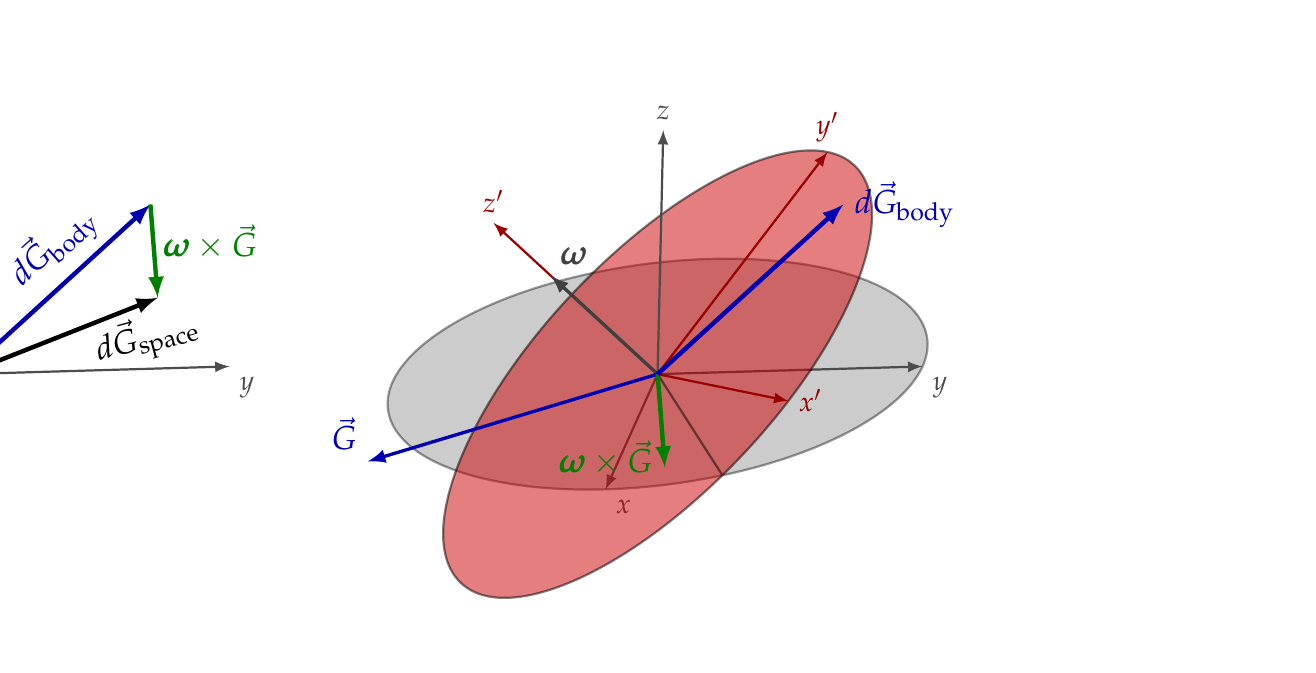
\begin{tikzpicture}[scale=0.8]
\useasboundingbox (-10.0,-4.3) rectangle (10.0,5.5);

% General parameters
\def\radius{4}      % Base plane radius
\def\rA{0.3}        % Small arc radius (for angle indicators)
\def\addAx{0}       % Extra axis length on top of radius (for arrows)
\def\thetaAngle{40} % theta Euler angle
\def\psiAngle{-20}  % psi Euler angle
\def\phiAngle{-25}  % phi Euler angle

% parameters of the vector
\def\Omradius{0.65}         % length of the omega vector (as fraction of radius)
\def\XposVect{-0.55*\radius} % x-position vector
\def\YposVect{-0.8*\radius} % y-position vector
\def\ZposVect{0.5*\radius} % y-position vector
% time change in body frame
\def\XdVect{0.0*\radius} % x-position vector
\def\YdVect{0.9*\radius} % y-position vector
\def\ZdVect{-0.2*\radius} % y-position vector

\colorlet{CustomBlue}{blue!70!black}
\colorlet{CustomGreen}{green!50!black}

\begin{scope}[xshift=-11cm, rotate around y =-55, rotate around x = -90, rotate around y = 5]



\begin{scope}[rotate around z = \phiAngle]
    % x-axis
    \draw[thick, -latex, color=gray!60!black] (0,0,0) -- (\radius+\addAx,0,0) node[below right] {$x$};

    % y-axis
    \draw[thick, -latex, color=gray!60!black] (0,0,0) -- (0,\radius+\addAx,0) node[below right] {$y$};
    
\end{scope}

% z-axis
\begin{scope}[rotate around z = \phiAngle]
    \draw[thick, -latex,color=gray!60!black] (0,0,0) -- (0,0,\radius) node[above] {$z$};
\end{scope}

% Scope of rotated body frame after nutation 
\begin{scope}[rotate around x = \thetaAngle]

    % final axes (x', y', z')
    \begin{scope}[rotate around z = -\psiAngle]

    \coordinate (EnddVect) at (\XdVect, \YdVect, \ZdVect);
    \coordinate (Endomega) at (-\YposVect*\Omradius, \XposVect*\Omradius, 0);
    \coordinate (EndtotVect) at ($(EnddVect) + (Endomega)$);
    
    % draw the vector in body-fixed frame
    \draw[ultra thick, -latex, CustomBlue]  (0,0,0) -- (EnddVect) node[pos=0.6, above, rotate=42, font=\large] {$d \vec{G}_{\text{body}}$};
    \draw[ultra thick, -latex, CustomGreen]  (EnddVect) -- (EndtotVect) node[pos=0.4, right, font=\large] {$\pmb{\omega} \times \vec{G}$};
    \draw[ultra thick, -latex]  (0,0,0) -- (EndtotVect) node[pos=0.9, below, rotate=15, font=\large] {$d \vec{G}_{\text{space}}$};
    \end{scope}
\end{scope}

\end{scope}



\begin{scope}[rotate around y =-55, rotate around x = -90, rotate around y = 5]

% Original plane
\draw[thick, fill=gray,opacity=0.4] (0,0) circle (\radius);


\begin{scope}[rotate around z = \phiAngle]
    % x-axis
    \draw[thick, -latex, color=gray!60!black] (0,0,0) -- (\radius+\addAx,0,0) node[below right] {$x$};

    % y-axis
    \draw[thick, -latex, color=gray!60!black] (0,0,0) -- (0,\radius+\addAx,0) node[below right] {$y$};
    
\end{scope}

% red nutation plane
\begin{scope}[rotate around x = \thetaAngle]
    \draw[thick, fill=red!80!black,opacity=0.5] (0,0,0) -- (\radius,0,0 ) arc (0:360:\radius);
\end{scope}

% z-axis
\begin{scope}[rotate around z = \phiAngle]
    \draw[thick, -latex,color=gray!60!black] (0,0,0) -- (0,0,\radius) node[above] {$z$};
\end{scope}

% Scope of rotated body frame after nutation 
\begin{scope}[rotate around x = \thetaAngle]

    % final axes (x', y', z')
    \begin{scope}[rotate around z = -\psiAngle]
    
    \draw[thick, -latex, red!60!black] (0,0,0) -- (\radius+\addAx,0,0) node[right] {$x'$};

    \draw[thick, -latex, red!60!black] (0,0,0) -- (0, 1*\radius, 0) node[above] {$y'$};
    
    \draw[thick, -latex, red!60!black] (0,0,0) -- (0,0,\radius+\addAx) node[above] {$z'$};

    % draw the vector in body-fixed frame
    \draw[very thick, -latex, gray!50!black]  (0,0,0) -- (0,0,\Omradius*\radius) node[above right, font=\large] {$\pmb{\omega}$};
    \draw[very thick, -latex, CustomBlue]  (0,0,0) -- (\XposVect, \YposVect, \ZposVect) node[above left, font=\large] {$\vec{G}$};
    \draw[ultra thick, -latex, CustomGreen]  (0,0,0) -- (-\YposVect*\Omradius, \XposVect*\Omradius, 0) node[left, pos=0.9, font=\large] {$\pmb{\omega} \times \vec{G}$};
    \draw[ultra thick, -latex, CustomBlue]  (0,0,0) -- (\XdVect, \YdVect, \ZdVect) node[right, font=\large] {$d \vec{G}_{\text{body}}$};
    \end{scope}
\end{scope}

\end{scope}


\end{tikzpicture}
\end{document}
